\chapter{Θεωρία πληροφοριών}
\label{chapter:chap3}

\section{Εισαγωγή}
\label{section:sect31}

\indent Σε αυτό το κεφάλαιο γίνεται μια εισαγωγή σε βασικά στοιχεία της Θεωρίας πληροφοριών και η επεξήγηση της έννοιας εντροπίας της πληροφορίας. Επίσης θα αναφερθούν αλγόριθμοι συμπίεσης (entropy encoding) καθώς και ο αλγόριθμος kmeans που χρησιμοποιήθηκε για την παραγωγή των codebooks.

\section{Εντροπία}
\label{section:sect32}

\indent Η εντροπία κατά Shannon που εισήχθηκε από τον Claude E. Shannon το 1948 είναι η ποσοτικοποίηση της αβεβαιότητας μιας τυχαίας μεταβλητής και συνήθως μετριέται σε bits ή nats. Η κύρια πληροφορία που παρέχεται από την εντροπία και είναι χρήσιμη σε εμάς είναι το απόλυτο κάτω όριο μέχρι το οποίο η πληροφορία μπορεί να συμπιεστεί. Η εντροπία ορίζεται ως $ H(X) = -\sum_{i=1}^{n} p(x_i)*\ log_{b} p(x_i) $  οπού $p(x_i)$ είναι η πιθανότητα του ενδεχομένου $x_i$ και η βάση b ορίζει την μονάδα μέτρησης της εντροπίας.Για την συμπίεση δεδομένων συνήθως ισχύει $b=2$, ώστε να έχουμε την εντροπία σε bits.

\indent Για να γίνει κατανοητή η έννοια της εντροπία θα δοθεί ένα παράδειγμα. Έστω ότι πρέπει να αναπαρασταθεί μια ακολουθία από αριθμούς $x_i \in [0,3] $ σε δυαδικό σύστημα. Επομένως υπάρχουν $n=4$ διαφορετικά ενδεχόμενα που χρειάζονται 2 bits το καθένα για να αναπαρασταθούν τα
$x_i = \begin{bmatrix}
0 & 0 \\
0 & 1 \\
1 & 0 \\
1 & 1
\end{bmatrix} $. Αν τα ενδεχόμενα είναι ισοπίθανα ισχύει ότι $ \forall{x_i}, p(x_i)= 0.25 $ και προκύπτει ότι $ H(X) = 2bits $. Συνεπώς, δε μπορεί να γίνει συμπίεση. Αν όμως ισχύει ότι $ p(x_1) = 0.7, p(x_2)=p(x_3)=p(x_4)=0.1 $ τότε έχουμε $ H(X) = 1.35678 bits$ ανά σύμβολο κατά μέσο όρο. Επομένως τα δεδομένα μας μπορούν ιδανικά να συμπιεστούν κατά $(1-1.35678/2)\% = 32\%$.

\section{Κωδικοποιητές Εντροπίας}
\label{section:sect33}

\indent Οι μέθοδοι που σήμερα υπάρχουν για συμπίεση καταφέρνουν να έρθουν πολύ κοντά στο όριο που δίνει η εντροπία αλλά δε το φτάνουν. Δύο είναι οι κυρίαρχες, η μέθοδος Huffman και Αριθμητική κωδικοποίηση. Η δεύτερη να είναι η πιο δημοφιλής περισσότερο στο βίντεο με την παραλλαγή της που λέγεται CABAC (Context Adaptive Binary Arithmetic Coding)
\begin{itemize}
  \item Η μέθοδος Huffman έχει την μικρότερη πολυπλοκότητα O(nlogn) μεταξύ των δυο και μας εξασφαλίζει πώς $ H(X) \leq HC \leq H(X)+1bit  $ όπου HC είναι το μέσο μήκος ανά σύμβολο που δίνει ο Huffman. Ο αλγόριθμος βάζει τα ενδεχόμενα σε ένα δυαδικό δέντρο και τους αναθέτει λέξεις με διαφορετικό μήκος. Στόχος είναι το ενδεχόμενο με την μεγαλύτερη πιθανότητα να έχει το μικρότερο μήκος και αυτό με την μικρότερη πιθανότητα το μεγαλύτερο μήκος. Έστω λοιπόν ότι έχουμε 5 ενδεχόμενα $x_i$ με πιθανότητες $p(S_0) = 0.5, p(S_1)=p(S_2)=0.2, p(S_3)=p(S_4)=0.05$. Το αντίστοιχο δέντρο Huffman για αυτό το παράδειγμα φαίνεται στο Σχήμα~\ref{fig:huffman}.
      \begin{figure}[h!]
          \centering
          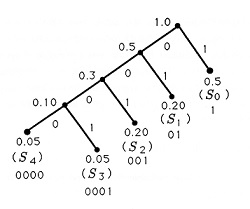
\includegraphics[width=0.5\textwidth]{chapter3/huffman.jpg}
          \caption{Δέντρο Huffman.}
          \label{fig:huffman}
      \end{figure}

\newpage
  \item Η μέθοδος της Αριθμητικής Κωδικοποίησης έχει την μεγαλύτερη πολυπλοκότητα μεταξύ των δύο αλλά μας εξασφαλίζει μια εν γένει καλύτερη συμπίεση από αυτή τού Huffman και αρκετά "κοντά" την εντροπία. Ο αλγόριθμος όπως και στον Huffman έχει στόχο να δώσει μεγάλο μήκος στα ενδεχόμενα με την μικρότερη πιθανότητα και μικρό σε αυτά με την μεγαλύτερη. Η διαφορά του με τον Ηuffman είναι πως δεν κωδικοποιεί ανά σύμβολο αλλά όλο την σειρά συμβόλων σε έναν μοναδικό αριθμό $n \in R$. Για παράδειγμα έστω μια κατανομή με 3 σύμβολα A,B,C και τις πιθανότητες τους $ p(A) = 0.5, p(B) = 0.33, p(C) = 0.17 $ και έστω το μήνυμα που κωδικοποιείται είναι το "BCA" . Στο Σχήμα~\ref{fig:ac} φαίνονται τα βήματα της κωδικοποίησης. Στο πρώτο βήμα έρχεται το B και το κωδικοποιούμε με τον αριθμό 0b01(x) γιατί έχει το μικρότερο μήκος και βρίσκεται στο [0.5,0.83) οπού x σημαίνει αυθαίρετη ακολουθία από bits. Έτσι συνεχίζουν και τα υπόλοιπα βήματα μέχρι να έχουμε τον αριθμό που αντιστοιχεί στην ακολουθία.

      \begin{figure}[ht!]
          \centering
          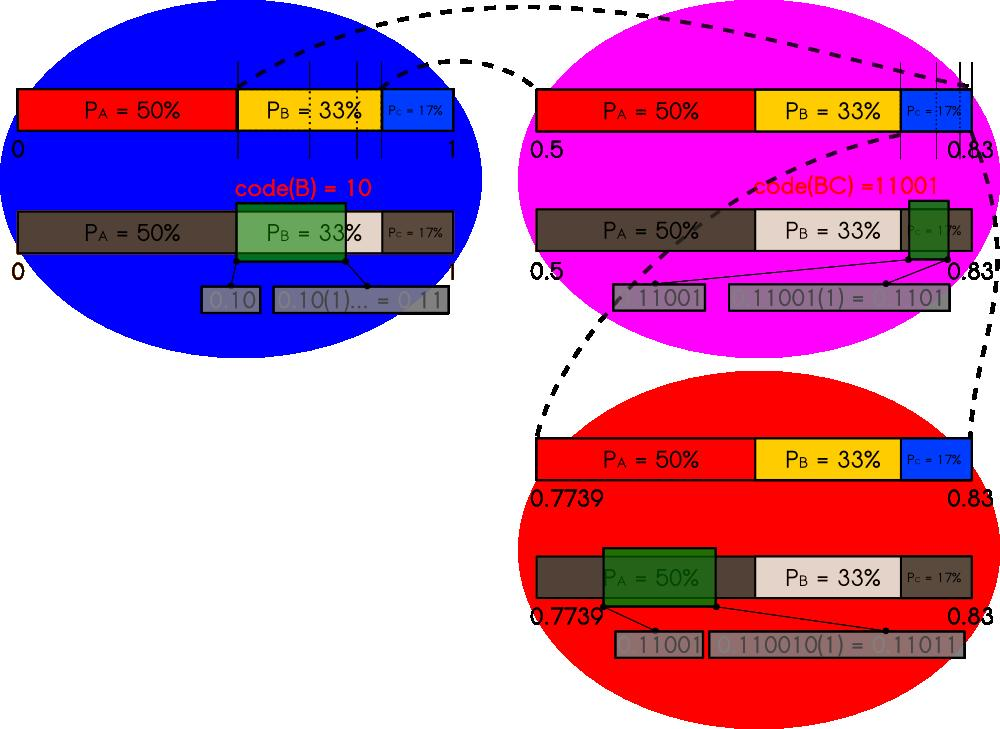
\includegraphics[width=0.5\textwidth]{chapter3/ac.jpg}
          \caption{Βήματα αριθμητικής κωδικοποίησης.}
          \label{fig:ac}
      \end{figure}
\end{itemize}

\newpage
\section{Αλγόριθμος clustering kmeans}
\label{section:sect34}

\indent Άλλο ένα στοιχείο που χρησιμοποιήθηκε σε αυτή την διπλωματική και πηγάζει από την Θεωρία πληροφοριών είναι ο αλγόριθμος clustering kmeans. Είναι ένας επαναληπτικός αλγόριθμος όπου στόχος του είναι να χωρίσει με το ελάχιστο σφάλμα n σημεία με διάσταση d σε k περιοχές $ k \leq n $ όπως φαίνεται στο Σχήμα~\ref{fig:kmeans}. O kmeans έχει πολύ μεγάλη υπολογιστική πολυπλοκότητα και ανάγεται στα προβλήματα NP-hard. Παρακάτω δίνεται σε ψευδοκώδικα ο αλγόριθμος.\\

\begin{algorithm}
\begin{algorithmic}[1]
\caption{K-Means pseudo code}
\label{alg:kmeans}
\STATE{Choose initial centers for clusters K;} \label{alg:kmeans:s1}
\WHILE{the clusters are changing}
    \STATE{Reassign the data points and set $Ktemp=0$;}
    \FORALL{Data points n} \label{alg:kmeans:s4}
        \STATE{Assign data point $n_i$ to the cluster $k_j$ whose center is closest;} \label{alg:kmeans:s5}
        \STATE{$Ktemp_j+=n_i$}
    \ENDFOR
    \STATE{Update the cluster centers;}
    \FOR{j:=1 to k step 1}
        \STATE{$\mathbf{r_j}$ = number of points in $Ktemp_j$;}
        \STATE{$\mathbf{K_j} = \frac{Ktemp_j}{r_j}$;}
    \ENDFOR
\ENDWHILE
\end{algorithmic}
\end{algorithm}
\begin{figure}[ht!]
  \centering
  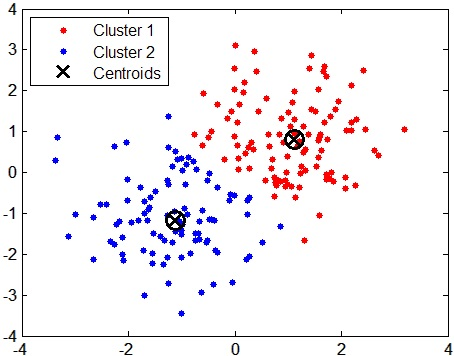
\includegraphics[width=0.5\textwidth]{chapter3/kmeans.jpg}
  \caption{kmeans με $k=2,d=2,n=100,MSE=284.671$}
  \label{fig:kmeans}
\end{figure}

\newpage

\indent Στο Βήμα ~\ref{alg:kmeans:s1} του Αλγορίθμου~\ref{alg:kmeans} γίνεται η αρχικοποίηση είτε με τυχαίο τρόπο (κάθε cluster να παίρνει τιμές από ένα τυχαίο point) είτε με κάποια στρατηγική. Στην παρούσα διπλωματική επιλέχθηκε η στρατηγική KKZ (Katsavounidis Kuo Zhang) η οποία έχει μεγαλύτερη πολυπλοκότητα από την τυχαία αλλά οδηγεί τον kmeans σε γρηγορότερη σύγκλιση και μικρότερο σφάλμα. Ο αλγόριθμος παραλληλοποιήθηκε με OpenMP και επιτεύχθηκε γραμμική επιτάχυνση. Στο Σχήμα~\ref{fig:kkzspeed} παρατίθεται η επιτάχυνση του παράλληλου αλγορίθμου και στο Σχήμα~\ref{fig:kkziter} οι συνολικές επαναλήψεις που κάνει ο kmeans με τυχαία και KKZ αρχικοποίηση.

\begin{figure}[ht!]
  \centering
  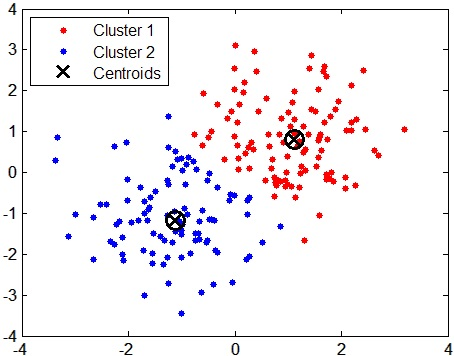
\includegraphics[width=0.5\textwidth]{chapter3/kmeans.jpg}
  \caption{kmeans με $k=2,d=2,n=100,MSE=284.671$}
  \label{fig:kkzspeed}
\end{figure}

\begin{figure}[ht!]
  \centering
  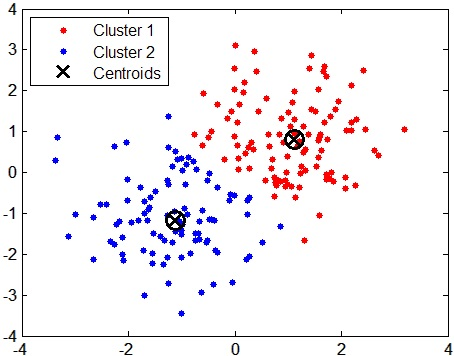
\includegraphics[width=0.5\textwidth]{chapter3/kmeans.jpg}
  \caption{kmeans με $k=2,d=2,n=100,MSE=284.671$}
  \label{fig:kkziter}
\end{figure}

\newpage

\indent Η πιο σημαντική βελτιστοποίηση επιτεύχθηκε στο σημείο της αναζήτησης του κοντινότερου cluster στο Βήμα~\ref{alg:kmeans:s5} του Αλγορίθμου~\ref{alg:kmeans}. Στην απλή εκδοχή του αλγορίθμου για κάθε data point σαρώνονται όλα τα clusters για να βρεθεί το κοντινότερο. Στην παρούσα διπλωματική, χρησιμοποιήθηκε ο αλγόριθμος Fast Nearest Neighbour ο οποίος οργανώνει τις αποστάσεις σε ένα δυαδικό δέντρο. Ο FastNN μας επιτρέπει να κάνουμε $ log_{2} k $  αναζητήσεις (πολυπλοκότητα αναζήτησης σε δυαδικό δέντρο), διαφορετικά θα έπρεπε να γίνουν k αναζητήσεις. Αυτό οδηγεί σε μεγάλη επιτάχυνση του προβλήματος της αναζήτησης που είναι το κύριο σημείο συμφόρησης του αλγορίθμου. Σε συνδυασμό με την παραλληλοποίηση στο Βήμα~\ref{alg:kmeans:s4} με OpenMP μας επέτρεψε να τρέχουμε μεγάλα πειράματα σε εύλογο χρονικό διάστημα. Οι επιταχύνσεις που επιτεύχθηκαν με την χρήση του FastNN παρουσιάζονται στο Σχήμα~\ref{fig:fastnn} και της παραλληλοποίησης του Βήματος 4 στο Σχήμα~\ref{fig:ompiter}

\begin{figure}[ht!]
  \centering
  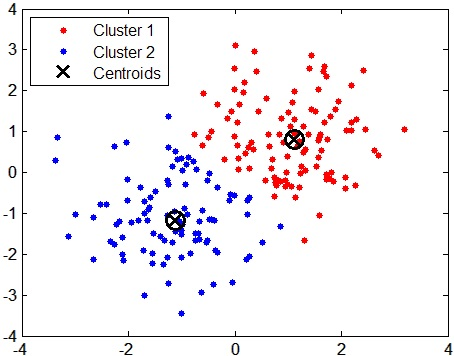
\includegraphics[width=0.5\textwidth]{chapter3/kmeans.jpg}
  \caption{kmeans με $k=2,d=2,n=100,MSE=284.671$}
  \label{fig:fastnn}
\end{figure}

\begin{figure}[ht!]
  \centering
  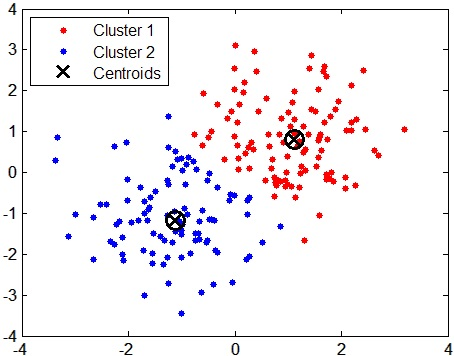
\includegraphics[width=0.5\textwidth]{chapter3/kmeans.jpg}
  \caption{kmeans με $k=2,d=2,n=100,MSE=284.671$}
  \label{fig:ompiter}
\end{figure}

\newpage
\indent Για τα πειράματα της διπλωματικής χρησιμοποιήθηκε o εξοπλισμός με τα ακόλουθα χαρακτηριστικά: 
\begin{itemize}
    \item HP Blade Server
    \item OS Microsoft Windows Server 2008 R2 Datacenter.
    \item CPU 2xIntel Xeon E5-2600 @ 2.30Ghz οπού παρείχαν συνολικά 12 Threads + 12 με HyperThreading.
    \item RAM 32GB.
\end{itemize} 